%\documentclass[12pt, twoside]{report}
\documentclass[12pt]{report}		

%%% CHOOSE THE COLOR SCHEME %%%
% User defined color which will be used throughout the document
% In case you want another color, find its HTML code (without #), a 6-digit string consisting of numbers and letters, then replace it in the brackets
\def\htmlmaincolorcode{607B8B} 
% Analogously, choose the color for shaded equation boxes, in case you wish to use them
\def\htmlshadecolorcode{E4EDF2}
% If you don't want any color and prefer black, just replace the option [customcolor] with [black]
\usepackage[customcolor]{ctp-fpub}


%%% ADD HERE ALL THE PACKAGES YOU USE %%%
% Packages required only for the specific content in this template, remove if not needed
\usepackage{slashed}
\usepackage{dsfont}


\bibliography{reference}


% If you want to compile just a part of the thesis use \includeonly
% For example:
% \includeonly{filename2,filename3}


%%% REPLACE THE INFORMATION IN THE BRACKETS %%%
% Information contained in the title page
\def\studentname{Name Surname} 
\def\thesistitle{Wilson Loops}
% In case of no subtitle, just leave this field empty {}
\def\thesissubtitle{Mundane primer for the uninitiated}
\def\thesistype{Bachelor}
\def\firstsupervisor{First Supervisor}
\def\firstsupervisorprefix{Prof. Dr.}
% In case of no second supervsior, just leave these fields empty {}
\def\secondsupervisor{Second Supervisor}
\def\secondsupervisorprefix{Lect. Dr.}
% In case of a third supervisor, well... 
\def\domeniu{Fizică Teoretică şi Computaţională}
\def\tipteza{licență}

\begin{document}

% Title page
\newgeometry{margin=1in}
\newcommand{\HRule}{\rule{\linewidth}{0.4mm}}

\begin{titlepage}
	\begin{center}


		\begin{tabular}{lcr}


			
\includegraphics[width=2.5cm]{unibuc.jpg} &

			\begin{tabular}{c}
				{\large \textsc{Universitatea din București}} \\
				{ \large \text{Facultatea de Fizică}}\\
				\\
				\\
				\\
				\\
				\\
			\end{tabular}
			& 
\includegraphics[width=3.3cm]{fizica}
		\end{tabular}


		\vspace{2cm}

		{\Large Sebastian MICLUȚA-CÂMPEANU}\\[1.1cm]

		\HRule \\[0.3cm]

\begin{spacing}{2}
	{\Large \bfseries {LASER WAKEFIELD ACCELERATION}}\\
	{\Large \bfseries Studies using Particle in Cell Method}
\end{spacing}

		\HRule \\[1.1cm]

		\textsc{\large Master Thesis}\\[3cm]

		\begin{minipage}{0.90\textwidth}
			\begin{flushright} \large
				{Scientific Advisers} \\[0.1cm]
				Prof.~dr.~Virgil BĂRAN \\
				Conf.~dr.~Alexandru NICOLIN
			\end{flushright}
		\end{minipage}

		\vfill

		{\large Bucharest, \the\year}

	\end{center}

\end{titlepage}

\restoregeometry

{\pagestyle{empty}\cleardoublepage}

\chapter*{Declaraţie}

Subsemnatul {\sffamily\color{maincolor}\studentname}, candidat la examenul de {\sffamily\color{maincolor}\tipteza} la Universitatea din București, Facultatea de Fizică, în domeniul {\sffamily\color{maincolor} Fizică}, programul de studii {\sffamily\color{maincolor}\domeniu}, declar pe propria răspundere că lucrarea de față este rezultatul muncii mele, pe baza cercetărilor mele și pe baza informațiilor obținute din surse care au fost citate și indicate, conform normelor etice, în note și în bibliografie. Declar că nu am folosit în mod tacit sau ilegal munca altora și că nici o parte din teză nu încalcă drepturile de proprietate intelectuală ale altcuiva, persoană fizică sau juridică. Declar că lucrarea nu a mai fost prezentată sub această formă vreunei instituții de învățămînt superior, în vederea obținerii unui grad sau titlu științific ori didactic.
\\[1cm]
Semnătura conducătorului lucrării,\hspace{4cm} Semnătura candidatului,

% You can add acknowledgments here
\chapter*{Acknowledgments}


\tableofcontents
{\pagestyle{empty}\cleardoublepage}
\addtocontents{toc}{\protect\thispagestyle{empty}}

\pagenumbering{arabic}

% Don't include the .tex extension for the file name with include.
\documentclass[12pt, class=report, crop=false]{standalone}
\usepackage{ba_thesis}

\begin{document}

% \addcontentsline{toc}{chapter}{Introduction}
\chapter{Introduction}%
\label{chap:intro}

In this thesis \dots

%\section*{Acknowledgments}
%I would like to thank my advisers, Prof.~dr.~Virgil Băran and Conf.~dr.~Alexandru Nicolin,
%for their help.

\end{document}

% Add chapters here
\chapter{QCD primer}
\label{chap:qcd}

Quantum chromodynamics is the theory of strong interactions\footnote{A brief historical review about the development of {\sffamily QCD} may be found at \cite{historyqcd}.}. It aims to describe the interactions between elementary constituents, namely the quarks\footnote{The quarks were firstly predicted in Gell-Mann's Eightfold Way \cite{gellmann}.}, mediated by the carriers of the color force, the gluons.

The existence of color charge was proposed as an additional quantum number which would solve the violation of Pauli's exclusion principle for some particular baryons\footnote{For example, $\Delta^{++}$, which consists of three up quarks.}. Since the quarks were never experimentally evidenced, it was proposed that the strong interaction constrains the free particles to only exist in color neutral states. This particularity of {\sffamily QCD} is known as color confinement. Nevertheless, in the partonic picture\footnote{Feynman proposed that high energy nuclei are made of elementary constituents, generically called partons \cite{partons}.}, deep inelastic scattering\footnote{{\sffamily DIS} is a process during which the structure of a hadron may be probed via interaction with, in general, a lepton.} experiments between an electron and a proton confirmed the already predicted Bjorken scaling\footnote{Bjorken deduced an expression for the cross-section of the electron by imagining that it interacts electromagnetically with each parton from the proton \cite{bjorkenimf}.} of the electrons' differential cross-section.

In essence, {\sffamily QCD} is an extension of the original $\textsf{SU}(2)$ gauge theory of Yang and Mills \cite{yangmills} to local non-Abelian $\textsf{SU}(3)$ gauge transformations.

\section{Field content}
Following textbook expositions \cite{maggiore, peskin, greiner}, the {\sffamily QCD} Lagrangian $\mathcal{L}$ is constructed from symmetry principles, namely $\textsf{SO}(1,3)$ Lorentz invariance and local gauge invariance under $\textsf{SU}(3)$. The fields should transform according to irreducible representations of these groups. The quark content of the Lagrangian is described by the quark and anti-quark fields $\psi_{\alpha,i,f}(x)$ and $\overline{\psi}_{\alpha,i,f}(x)$. They are Dirac spinors (spinorial index $\alpha$), transform according to the fundamental representation of $\textsf{SU}(3)$ (color index $i=1,2,3$ or red, green, blue) and come in different flavours (flavour index $f=\overline{1,N_f}$ or up, down, strange, charm, bottom, up). The gluon fields $A_a^\mu(x)$ are Lorentz vectors and each correspond to a generator $t^a$ ($a=\overline{1,8}$) which, in the fundamental representation, is given by the Gell-Mann matrices $t^a=\lambda^a/2$.

\section{Gauge transformations} 
The quark and anti-quark fields must be invariant under local $\textsf{SU}(3)$ gauge transformations\footnote{For simplicity, all the field indices will be dropped in the following computations.}
\shadedeq{
    \psi(x)\mapsto\textsf{U}(x)\psi(x), \quad \overline{\psi}\mapsto\overline{\psi}(x)\textsf{U}^\dagger(x) 
}
with the group transformation expressible, via exponentiation, from the Lie algebra generators, with space-time dependent group parameters $\varepsilon^a(x)$, as 
\boxedeqlabel{gaugetransf}{
    \textsf{U}(x)=\exp{i\sum_a\varepsilon^a(x)t^a}
}
The gauge fields\footnote{For each algebra element $t^a$, one may introduce a gauge field $A_a^\mu$. These may be then used to construct a Lie-algebra valued gauge potential $A^\mu$. This potential depends on the chosen representation.} $A_\mu(x)=\sum\limits_a A^a_\mu(x)t^a$ must transform according to
\boxedeqlabel{gaugefields}{
    A_\mu(x)\mapsto\textsf{U}(x)A_\mu(x)\textsf{U}^\dagger(x)+\frac{i}{g}\textsf{U}(x)\big[\partial_\mu\textsf{U}^\dagger(x)\big]
}
where $g$ denotes the coupling constant. It is important to notice that one may generate gluon fields out of a null one, that is $A_\mu=0$ by applying a local gauge transformation. Such field configurations take the form
\begin{equation*}
    A_\mu^{\text{pure}}=\frac{i}{g}\textsf{U}\big(\partial_\mu\textsf{U}^\dagger\big)
\end{equation*}
and are called pure gauge fields \cite{gelisqft,eichmann}. The corresponding field strength tensor is null $F_{\mu\nu}^{\text{pure}}=0$.

One may introduce the covariant derivative\footnote{The covariant derivative has an elegant geometrical interpretation \cite{torre}: it represents the rate of change when fields from different space-time points are parallel transported along a given path. During this procedure, they are being aligned such that they may be properly compared. The corresponding connection is actually the gauge field.}
\begin{equation*}
    \textsf{D}_\mu=\partial_\mu-igA_\mu. 
\end{equation*}
Further, one may define the field strength tensor as the commutator between covariant derivatives\footnote{Since it arises as a commutator between covariant derivatives, which describe the parallel transport, the field strength tensor may be interpreted as a measure of the path dependence of parallel transport. For this reason, it is also referred to as the curvature \cite{torre}.}
\begin{equation*}
    F_{\mu\nu}=\frac{i}{g}\big[\textsf{D}_\mu,\textsf{D}_\nu\big],
\end{equation*}
which yields an expression in terms of gauge fields
\shadedeq{
    F_{\mu\nu}=\partial_\mu A_\nu-\partial_\nu A_\mu-ig\big[A_\mu,A_\nu\big]
}
or equivalently, by color components $F_{\mu\nu}=F_{\mu\nu}^at^a$, as
\begin{equation*}
    F_{\mu\nu}^a=\partial_\mu A_\nu^a-\partial_\nu A_\nu^a+gf^{abc}A_\mu^bA_\nu^c,
\end{equation*}
where $f^{abc}$ are the structure constants of the Lie algebra $\mathfrak{su}(3)$. The last term from the above equation, when plugged in the Lagrangian, will give rise to gluonic self-interactions, a particular feature of QCD. The field strength tensor gauge transforms in the usual manner as
\shadedeq{
    F_{\mu\nu}(x)\mapsto \textsf{U}(x)F_{\mu\nu}(x)\textsf{U}^\dagger(x)
}

\section{QCD Lagrangian} 
One may now proceed to constructing the Lagrangian. The quark content is that of a free fermionic Lagrangian\footnote{After replacing the partial derivative with the covariant derivative, the Lagrangian will also contain an interaction term
\begin{equation*}
    \mathcal{L}_{\textsf{int}}=g \overline{\psi} \gamma^\mu A_\mu^a t^a \psi.
\end{equation*}}, but built with covariant derivatives, in order to satisfy gauge invariance
\begin{equation*}
    \mathcal{L}_{\textsf{quarks}}=\overline{\psi}(x)\big(i\slashed{\textsf{D}}-\textsf{M}\big)\psi(x),
\end{equation*}
where $\textsf{M}=\textsf{Diag}\left\{m_1,\ldots,m_{N_f}\right\}$ is the diagonal quark mass matrix in flavour space\footnote{In the Standard Model, the quark mass matrix is no longer diagonal. After spontaneous symmetry breaking, the mixing between different flavoured quark masses is given by the {\sffamily CKM} matrix \cite{pdg}.}. 

The dynamics of the gluon fields is described by the following construction\footnote{It is important to notice that such a construction contains not only standard kinetic terms but also interaction vertices with three gluons, which are proportional to $g$ and four gluons, proportional to $g^2$.}
\begin{equation*}
    \mathcal{L}_{\textsf{gluons}}=-\frac{1}{2}\textsf{Tr}\left\{F_{\mu\nu}F^{\mu\nu}\right\},
\end{equation*}
where the color tracing over the contraction of field strength tensors assured gauge invariance. Equivalently, one may rewrite the above expression in terms of color components as
\begin{equation*}
    \mathcal{L}_{\textsf{gluons}}=-\frac{1}{4}F_{\mu\nu}^aF^{a,\mu\nu},
\end{equation*}
valid in the fundamental representation, where $\textsf{Tr}\left\{t^at^b\right\}=\delta^{ab}/2$. Therefore, the {\sffamily QCD} Lagrangian takes the form
\boxedeqlabel{qcd6}{
    \mathcal{L}_{\textsf{QCD}}=\overline{\psi}(x)\big(i\slashed{\textsf{D}}-\textsf{M}\big)\psi(x)-\frac{1}{4}F_{\mu\nu}^aF^{a,\mu\nu}
}

The corresponding Yang-Mills action expressed in flat coordinates is given by
\begin{align}\label{yangmills}
    \textsf{S}=\int\mathrm{d}^4x\left(-\frac{1}{2}\textsf{Tr}\left\{F_{\mu\nu}F^{\mu\nu}\right\}\right),
\end{align}

\section{Field equations} 
The variational derivatives with respect to the color spinor fields give the colored Dirac equations
\begin{equation*}
    (i\slashed{\textsf{D}}-\textsf{M})\psi=0,    
\end{equation*}
and similarly for the anti-quark fields
\begin{equation*}
    \overline{\psi}(i\overleftarrow{\slashed{\textsf{D}}}-\textsf{M})=0.    
\end{equation*}
The Euler-Lagrange equations corresponding to the gluon fields yield the Yang-Mills equations, or equivalently, colored Maxwell equations\footnote{There is an additional equation, called the Bianchi identity, which follows from the definition and properties of $F_{\mu\nu}$. It may be expressed as \cite{tong}
\begin{equation*}
    \textsf{D}_\mu^{\phantom{*}*}F^{\mu\nu}=0,
\end{equation*}
where we introduced the dual field strength tensor as
\begin{equation*}
    ^*F^{\mu\nu}=\frac{1}{2}\epsilon^{\mu\nu\rho\sigma}F_{\rho\sigma}.
\end{equation*}}
\shadedeq{
    \textsf{D}_\nu F^{\nu\mu}=gJ^\mu
}
in which $J^\mu=\sum\limits_a J^{a,\mu} t^a$ with $J^{a,\mu}=\overline{\psi}\gamma^\nu t^a\psi$ being the color current. The color current is covariantly conserved $\textsf{D}_\mu J^\mu=0$.

\chapter{Lattice gauge theory}
\label{chap:latticeqcd}

\section{Gauge invariance} 
Nevertheless, a naive discretization of the Yang-Mills action from Equation \cref{yangmills}, in which one replaces all the partial derivatives appearing in the field strengths $F^{\mu\nu}$ with finite differences leads to the loss of gauge invariance \cite{schwartz, peskin}. 

\begin{remark}
This is a consequence of imposing local gauge symmetry, with a $\textsf{SU}(3)$ gauge transformation given by Equation \cref{gaugetransf}, of the fields
\begin{align*}
    \phi(x)\mapsto \textsf{U}(x)\phi(x).
\end{align*}
Fields at different space-time points cannot directly be compared. Because of this, the partial derivative, which contains the difference between fields at different points, is not well defined. By introducing a quantity which gauge transform as
\begin{align}\label{latt3}
    \textsf{W}(x,y)\mapsto\textsf{U}(x)\textsf{W}(x,y)\textsf{U}^\dagger(y),
\end{align}
one may now properly define the covariant derivative as\footnote{Notice that with this definition, the covariant derivative transforms as
\begin{align}\label{latt1}
    \textsf{D}_\mu\phi(x)\mapsto\textsf{U}(x)\textsf{D}_\mu\phi(x).
\end{align}
}

\begin{definition}[Covariant derivative]
\begin{align}\label{latt2}
    \textsf{D}_{\mu} \phi(x)\overset{\Delta}{=} \lim _{\delta \epsilon^{\mu} \rightarrow 0} \frac{\textsf{W}(x, x+\epsilon) \phi(x+\epsilon)-\phi(x)}{\epsilon^\mu}.
\end{align}
\end{definition}
\noindent We choose $\textsf{W}(x,x)=\mathds{1}$ and then write an expansion in terms of the gauge fields\footnote{If we plug in this relation back in Equation \cref{latt2} and then in Equation \cref{latt1}, we deduce the gauge transformation of the gauge fields from Equation \cref{gaugefields}.}
\begin{align*}
    \textsf{W}(x,x+\epsilon)=1+ig\epsilon^\mu A_\mu+\mathcal{O}(\epsilon^2).
\end{align*}
\end{remark}

This enables us to express the {\sffamily\color{maincolor}Wilson line} as\footnote{Where the fields may further be written as $A_{\mu}=A_{\mu}^aT^a$ in the fundamental representation.}
\boxedeqlabel{latt5}{
    \textsf{W}(x,y)=\mathcal{P}\exp{i g \int_{y}^{x} \mathrm{d} z^{\mu} A_{\mu}(z) }
}

\begin{remark}
The {\sffamily\color{maincolor}path-ordering} operator $\mathcal{P}\{\ldots\}$ is necessary due to the non-Abelian nature of the fields. More clearly, after writing a Taylor expansion, the path-ordering operator acts as

\begin{align*}
    \begin{aligned}
    \textsf{W}(x, y)=& 1+i g \int_{0}^{1} \frac{\mathrm{d} z^{\mu}_\lambda}{\mathrm{d} \lambda} A_{\mu}^{a}(z_\lambda^\mu) T^{a} \mathrm{d} \lambda-\frac{1}{2} g^{2} \int_{0}^{1} \mathrm{d} \lambda \int_{0}^{1} \mathrm{d} \tau \frac{\mathrm{d} z^{\mu}_\lambda}{\mathrm{d} \lambda} \frac{\mathrm{d} z^{\nu}_\tau}{\mathrm{d} \tau}\times\\
    & \times A_{\mu}^{a}(z_\lambda^\mu) A_{\nu}^{b}(z_\tau^\nu)\left[T^{a} T^{b} \theta(\lambda-\tau)+T^{b} T^{a} \theta(\tau-\lambda)\right]+\cdots.
\end{aligned}
\end{align*}
\end{remark}

A Wilson line taken along a closed path $\gamma$ is called a {\sffamily\color{maincolor}Wilson loop} and it's given by
\boxedeqlabel{latt4}{
    \textsf{W}_\gamma=\mathcal{P}\exp{i g \oint\limits_{\gamma} \mathrm{d} x^{\mu} A_{\mu}(x)}
}

It is important to emphasize that the trace of a Wilson loop is gauge invariant\footnote{This may easily be proven by inserting Equation \cref{latt4} back in Equation \cref{latt3} and using the invariance of the trace under cyclic permutations.}.

\section{Real-time lattice gauge theory} 
Let us begin by discretizing the Minkowski space-time on a hypercubic lattice\footnote{The lattice spacing along direction $\mu$, with the unit vector is $\hat{e}^\mu$, is $a^\mu$. This enables us to write $\hat{a}^{\mu}=a^\mu\hat{e}^\mu$. More concisely, $a^0$ is the time step and $a^i$ denote the spatial lattice spacings.} whose points are given by
\begin{align*}
    \textsf{X}^4=\left\{x \mid x=\sum_{\mu=0}^{3} n_{\mu} \hat{a}^{\mu}, \quad n_{\mu} \in \mathbb{Z}\right\}.
\end{align*}

A field $\phi(x)$ which resides on the lattice will be denoted as $\phi_x$, with $x\in\textsf{X}^4$. The gauge transformation $\textsf{U}(x)$ will become, upon discretization, $\textsf{U}_x$. The discretized action and corresponding field equations written in terms of $A_\mu$ will not remain gauge invariant.

Nevertheless, a gauge invariant lattice action may be constructed. Instead of using the gauge fields $A_\mu$, along with the corresponding conjugate momenta $P_\mu$, as the main degrees of freedom, one may simply seek for a more suitable quantity which is already gauge invariant and preserves gauge invariance upon discretization. An action built from such a quantity will inherently be gauge invariant. The simplest choice is the trace of a Wilson line, as given in Equation \cref{latt4}. We already saw that such a construction is gauge invariant.

\begin{figure}
    \centering
    \subfloat[\centering {\sffamily 2d} plaquette]{{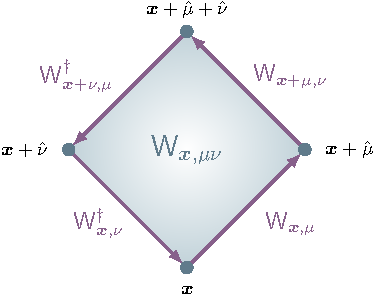
\includegraphics[width=0.45\textwidth]{plaquette_2d.pdf} }}%
    \qquad
    \subfloat[\centering {\sffamily 3d} plaquette]{{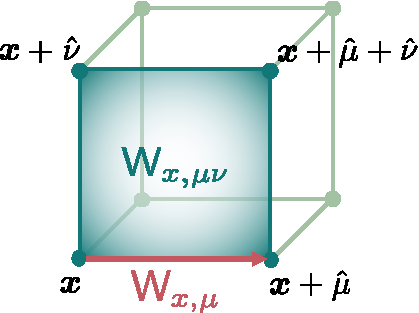
\includegraphics[width=0.45\textwidth]{plaquette_3d.pdf} }}%
    \caption{Schematic representations of a plaquette, the shortest Wilson loop on a rectangular lattice.}%
    \label{fig:plaquettes}%
\end{figure}

A Wilson line taken between two neighboring lattice points, namely $x$ and $x+\hat{a}^{\mu}$, is called a {\sffamily\color{maincolor}gauge link} and it's given by\footnote{Here $\overline{\mathcal{P}}\{\ldots\}$ denotes the anti-path-ordering. We introduce the notation
\begin{align*}
    \textsf{W}_{x,\mu}\overset{\Delta}{=}\textsf{W}(x,x+\hat{a}^{\mu})
\end{align*}
and similarly for $A_{x,\mu}$.
}
\begin{align*}
    \textsf{W}_{x, \mu}=\overline{\mathcal{P}} \exp{i g \int\limits_{x}^{x+\hat{a}^{\mu}} d x^{\mu} A_{x,\mu}}.
\end{align*}

\begin{remark}
In a similar manner, we may also introduce a gauge link along the opposite direction, which would yield
\begin{align}\label{latt6}
    W_{x,\mu}^{\dagger}=\textsf{W}_{x+\mu,-\mu}.
\end{align}
A gauge link transforms as
\begin{align*}
    \textsf{W}_{x, \mu} \rightarrow \textsf{U}_{x} \textsf{W}_{x, \mu} \textsf{U}_{x+\mu}^{\dagger}.
\end{align*}
One may express a gauge link and afterwards expand it, see Equation \cref{latt5}, as
\begin{equation*}
    \begin{aligned}
     \textsf{W}_{x,\mu}&=\exp{iga^\mu A_{x,\mu}}\approx \mathds{1}+iga^\mu A_{x,\mu(x)}-\frac{1}{2}g^2a^\mu a^\nu A_{x,\mu}A_
     {x,\nu}+\mathcal{O}(a^3).
\end{aligned}
\end{equation*}
\end{remark}

The simplest non-trivial\footnote{The shortest Wilson line would just go back and forth between two neighbouring sites but such a combination would simply yield the trivial result
\begin{align*}
    \textsf{W}_{x,\mu}\textsf{W}_{x+\mu,-\mu}\stackrel{\text{\cref{latt6}}}{=\joinrel=}\mathds{1}.
\end{align*}
} Wilson loop on the lattice may be constructed along the path connecting neighbouring points on a rectangular {\sffamily\color{maincolor}plaquette}, see Figure \cref{fig:plaquettes}, as
\begin{align*}
    \textsf{W}_{x, \mu \nu}&=\textsf{W}_{x, \mu} \textsf{W}_{x+\mu, \nu} \textsf{W}^\dagger_{x+\mu,\mu}\textsf{W}^\dagger_{x,\nu}\\
    &\stackrel{\text{\cref{latt6}}}{=\joinrel=}\textsf{W}_{x, \mu} \textsf{W}_{x+\mu, \nu} \textsf{W}_{x+\mu+\nu,-\mu} \textsf{W}_{x+\nu,-\nu},
\end{align*}
which may further be expressed as
\begin{align*}
    \textsf{W}_{x, \mu \nu} \approx \exp{ig a^{\mu} a^{\nu} F_{x,\mu \nu}+\mathcal{O}\left(a^{3}\right)}.
\end{align*}

\begin{proof}
We may write the discretized Wilson loop as\footnote{
Using the Campbell-Baker-Hausdorff formula
\begin{align*}
    \exp{\textsf{A}}\exp{\textsf{B}}\approx\exp{\textsf{A}+\textsf{B}+\frac{1}{2}[\textsf{A}, \textsf{B}]+\cdots}.
\end{align*}
}
\begin{align*}
    \textsf{W}_{x,\mu\nu}&\approx\exp\Bigg\{ig(A_{x,\mu}+A_{x+\mu,\nu}-A_{x+\nu,\mu}-A_{x,\nu})+\\
    &\phantom{\approx\exp\Bigg\{}+\frac{g^2}{2}\Big(\big[A_{x,\nu}+A_{x+\nu,\mu},A_{x+\mu,\nu}+A_{x,\mu}\big]-\\
    &\phantom{\approx\exp\Bigg\{}-\big[A_{x,\nu},A_{x+\nu,\mu}\big]-\big[A_{x+\mu,\nu},A_{x,\mu}\big]\Big)\Bigg\}.
\end{align*}
By making use of the expansion 
\begin{align*}
    A_{x+\mu,\nu}\approx A_{x,\nu}+a^\mu\partial_\mu A_{x,\nu}+\mathcal{O}(a^2),   
\end{align*}
we may then derive
\begin{align*}
     \textsf{W}_{x,\mu\nu}&\approx\exp\Big\{iga^\mu a^\nu\underbrace{\big(\partial_\mu A_{x,\nu}-\partial_\nu A_{x,\mu}-ig[A_{x,\nu},A_{x,\mu}]\big)}_{\mathclap{\textstyle F_{x,\mu\nu}}}+\mathcal{O}(a^3)\Big\}.
\end{align*}
This may further be approximated as
\begin{align*}
    \textsf{W}_{x,\mu\nu}=\mathds{1}+ig a^\mu a^\nu F_{x,\mu \nu}-\frac{1}{2}(ga^\mu a^\nu)^2 F_{x,\mu \nu}^2+\mathcal{O}(a^5).
\end{align*}
in the limit of small lattice spacings.
\end{proof}

Therefore, we may construct a gauge invariant quantity, since in contains Wilson lines traced over, under the discretized gauge transformation $\textsf{U}_x$ as

\begin{align}\label{latt7}
    \textsf{Tr}\big\{2-\textsf{W}_{x, \mu \nu}-\textsf{W}_{x, \mu \nu}^{\dagger}\big\} \approx\left(g a^{\mu} a^{\nu}\right)^{2} \textsf{Tr}\big\{F_{x,\mu \nu}^{2}\big\}+\mathcal{O}(a^{6}).
\end{align}

The Yang-Mills action from Equation \cref{yangmills} may be split into an electric and a magnetic part
\begin{align*}
    \textsf{S}=\underbrace{\int \mathrm{d}^{4}x \sum_{i}\textsf{Tr}\big\{F_{0i}^2(x)\big\}}_{\mathclap{\textstyle \textsf{S}_\textsf{E}}}+\underbrace{\int \mathrm{d}^{4}x\sum_{i, j} \frac{1}{2} \textsf{Tr}\big\{F_{ij}^2(x)\big\}}_{\mathclap{\textstyle \textsf{S}_\textsf{B}}}.
\end{align*}
Upon discretization, they become\footnote{By making the replacement
\begin{align*}
    \int \mathrm{d}^{4}x(\ldots)\mapsto \underbrace{\prod\limits_{\mu}a^\mu}_{\mathclap{\textstyle \textsf{V}}}\sum_x(\ldots)
\end{align*}
and using the result from Equation \cref{latt7}.
}
\begin{align*}
    \textsf{S}_\textsf{E}& \approx V \sum_{x} \sum_{i} \frac{1}{\left(g a^{0} a^{i}\right)^{2}} \textsf{Tr}\big\{2-\textsf{W}_{x, 0 i}-\textsf{W}_{x, 0 i}^{\dagger}\big\}, \\
    \textsf{S}_\textsf{B}& \approx V \sum_{x} \sum_{i, j} \frac{1}{2\left(g a^{i} a^{j}\right)^{2}} \textsf{Tr}\big\{2-\textsf{W}_{x, i j}-\textsf{W}_{x, i j}^{\dagger}\big\}.
\end{align*}
Thus, the Yang-Mills action on the lattice is given by

\shadedeq{
\textsf{S}=V \sum_{x}\Big( \sum_{i} \frac{1}{\left(g a^{0} a^{i}\right)^{2}} \textsf{Tr}\big\{2-\textsf{W}_{x, 0 i}-\textsf{W}_{x, 0 i}^{\dagger}\big\} -\sum_{i, j} \frac{1}{2\left(g a^{i} a^{j}\right)^{2}}\textsf{Tr}\big\{2-\textsf{W}_{x, i j}-\textsf{W}_{x, i j}^{\dagger}\big\}\Big)
}

\documentclass[../thesis.tex]{subfiles}

%!TeX spellcheck = en-GB

\begin{document}

\chapter{Conclusions}

In this thesis we have studied ...

\end{document}


\printbibliography


\end{document}
